\chapter{Implementatie}

In het adviesrapport zijn een vijftal adviezen opgesteld, die ik puntsgewijs behandel, zodat een goed beeld wordt verkregen van wat er gebeurd is bij Fullmoon.

\section{SCM Systeem}

\subsection{Keuze}

Bij het selecteren van het voor Fullmoon meest geschikte {\sc scm} systeem, hebben we rekening gehouden met meerdere eisen. Zo was één van de uitgangspunten dat de nieuwe situatie eenvoudig werkbaar moest zijn voor zowel alle in dienst zijnde medewerkers, als voor nieuwe medewerkers. Het moest dus een niet té ingrijpende verandering veroorzaken.

Omdat het een diverse groep is van designers, programmeurs en projectmanagers, waarbij niet iedereen zich even op het gemak voelt met de commandline, is bij Fullmoon gekozen voor Subversion. Het grote aanbod aan (grafische) tools gaf hierbij de doorslag.

\subsection{Uitwerking}

Bij Fullmoon zijn presentaties en uitleg gegeven over het werken met Subversion door gebruik te maken van het programma SmartSVN. Maar de medewerkers zijn in principe vrij in de keuze voor een programma om met Subversion te werken.

Er is een server in gebruik genomen om de Subversion repository te huisvesten. Op dezelfde server draait ook een webserver waarop alle projecten terug te zien zijn. Door middel van \emph{post-commit hooks} worden deze projecten automatisch bijgewerkt na elke commit. Zo is er een centrale plek waar iedereen de laatste versie van het project kan bekijken om deze eventueel te testen. Ook is dit handig om snel een website te kunnen bekijken zonder alles binnen te hoeven halen.

\subsection{Koppeling}

Naast het feit dat elke medewerker nu werkt met Subversion komt het ook nog in andere gebieden terug. Zo wordt er gebruik gemaakt van Subversion om code naar verschillende omgevingen te deployen en is er een centrale website ingericht om de activiteit van projecten te kunnen bekijken. Dit is na te lezen in respectievelijk sectie 2.2 en 2.4.

\section{Ontwikkelstraat}

Toen ik met mijn stage begon bij Fullmoon werd er gebruik gemaakt van twee verschillende omgevingen, één interne webserver waar op ontwikkeld werd en een externe server waar alle sites op draaiden. Dat aantal is verdubbeld tot vier door een acceptatie- en testomgeving toe te voegen. De huidige situatie is dus in de vorm van een OTAP-straat\footnote{ontwikkel, test, acceptatie en productie}. Er wordt niet voor elk project gebruik gemaakt van de acceptatieomgeving maar in principe gaat nieuwe code alle drie de omgevingen door voor het online komt te staan.

De ontwikkelomgeving is verplaats van de centrale server naar de workstations van de medewerkers zelf. Door middel van Subversion werkt iedereen nu op zijn eigen computer, zodat iedereen individueel kan werken aan projecten zonder elkaar hierbij in de weg zitten. Door middel van Subversion zijn de wijzigingen van anderen uiteraard nog wel binnen te halen.

Zoals vermeld in 2.1.2 wordt de testomgeving automatisch bijgewerkt in navolging van een commit. Hier kan een project intern getest worden door alle medewerkers. Omdat niet iedereen binnen Fullmoon direct aan projecten werkt, kan men van deze omgeving gebruik maken om projecten te kunnen bekijken zonder dat ze deze op hun eigen computer binnen te hoeven halen.

De acceptatieomgeving is ook een interne webserver die afgeschermd is voor de buitenwereld door middel van een gebruikersnaam en wachtwoord. Klanten kunnen hierop inloggen om bijvoorbeeld wijzigingen aan een site te beoordelen voordat deze online komt. Door middel van Subversion wordt een bepaalde versie van het project een \emph{tag} meegegeven, zodat de acceptatieomgeving de website kan tonen op basis van deze tag. Zo kan er verder gewerkt worden aan het project terwijl er controle is over welke versie de klant te zien krijgt om wijzigingen goed te keuren.

\section{Backup}

Bij Fullmoon was de backupsituatie al vrij goed geregeld. Intern worden van alle servers dagelijks backups gemaakt die bewaard worden op een externe hardeschijf. Online verzorgt de hostingprovider elke nacht de backups, deze worden een maand lang bewaard op een externe locatie maar blijven ook op de server zelf beschikbaar. Dit is handig om bijvoorbeeld snel een database te kunnen herstellen mocht er iets fout mee gegaan zijn.

Voor dit onderdeel heb ik weinig kunnen betekenen voor Fullmoon, omdat de situatie al ruim voldoende was ingericht. Alleen bij een calamiteit, zoals bij brand waar ik in het adviesrapport over heb gesproken, is het risico dat alle data verloren gaat nog steeds aanwezig. Daarom adviseer ik nadrukkelijk om deze backups niet op kantoor te bewaren, maar bij voorkeur offsite, dus op een andere lokatie. Over deze oplossing zijn we nog in overleg.

\section{Ticketsysteem}

Na vele systemen uitgeprobeerd te hebben is de keuze gevallen op Redmine. Deze sloot nauw aan bij de wensen van Fullmoon. Zo moest er een centrale plek komen waar de status van projecten te bekijken was, zowel issues als wijzigingen in de code.

Fullmoon gebruikt dit systeem op het moment alleen intern. Men levert sinds kort wel support aan de klant door middel van een ander ticketsysteen, maar dat staat los van Redmine. Mail naar een support-adres wordt door dit systeem opgevangen, waarna klanten verdere correspondentie en updates ook via de bijbehorende support-website kunnen raadplegen. In de toekomst zal nog geëvalueerd worden of het gebruik van twee systemen naast elkaar wel effectief is, aangezien Redmine voor beide doeleinden kan worden gebruikt.

\section{Automatisch deployen}

Om code naar verschillende omgevingen toe te sturen wordt gebruik gemaakt van Capistrano, in combinatie met de in het advies genoemde multistage plugin. Zo kan met één enkel commando code vanuit de Subversion repository naar de gewenste omgeving gestuurd worden.

Voordat hier gebruik van werd gemaakt ging het updaten van websites niet altijd even goed. Wanneer door meerdere personen lang aan een opdracht was gewerkt, was het vaak onduidelijk wat nou precies was gewijzigd en wat geupload moest worden. Zo kwam het regelmatig voor dat sommige functies niet goed werkten, omdat er een bepaald bestand ontbrak of dat het verkeerde bestand was geupload. Nu worden sites zonder gevaar en moeite geupdate, en is het een tamelijk eenvoudige handeling geworden, waar niet meer naar omgekeken hoeft te worden.

Door de samenwerking met Subversion biedt Capistrano ook de mogelijkheid om eenvoudig na te gaan welke versie van een project online staat. Voordat hiervan gebruik gemaakt kon worden was het giswerk wat er allemaal online stond, maar nu is direct zichtbaar vanaf welke revisie een website draait. 

\section{Vergelijking oude en nieuwe situatie}

\begin{figure}
  \centering
  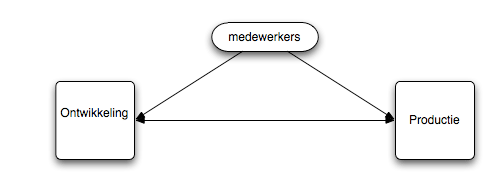
\includegraphics[scale=0.70]{situatie_oud.png}
  \caption[Oude situatie.]{De oude werksituatie bij Fullmoon.}
\end{figure}

\begin{figure}
  \centering
  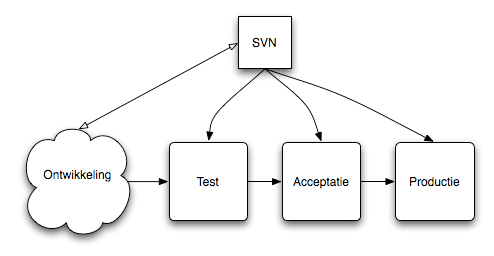
\includegraphics[scale=0.70]{situatie_nieuw.png}
  \caption[Nieuwe situatie.]{De nieuwe situatie.}
\end{figure}

In figuren 2.1 en 2.2 zijn respectievelijk de oude en nieuwe werksituatie bij Fullmoon grafisch uitgewerkt, ik geef hierover een kleine uitleg.

In de oude situatie werkte iedere medewerker via de eigen computer direct op de centrale ontwikkelserver, waarbij men vaak dezelfde bestanden open had staan. Soms werd er ook direct gewerkt op de onlineserver, waardoor er natuurlijk verschillen ontstonden.

In de nieuwe situatie werkt men op zijn eigen computer met gebruikmaking van Subversion (SVN). De ontwikkelomgeving in dit figuur bestaat dus in feite uit de computers van alle medewerkers. Wijzigingen gaan eerst de test- en acceptatieomgevingen door, voordat deze online komen te staan. Er worden dus alleen bestanden aangepast in de ontwikkelomgeving, zodat er nooit verschillende versies onstaan omdat iemand online wat heeft aangepast.